\subsection{Assignment: Newton's Method}
This method is a standard way in mathematics to find zeros of a function numerically. Graphically speaking, one computes the zero-crossing point of a tangent to a point on the function itself in each iteration. The projection of the zero onto the function serves as the new starting point in the following iteration. In each step, the algorithm approximates the zero more precisely until the method is aborted below a certain error.
For the exercise, the starting point (\ref{eq:start}) for a function (\ref{eq:fun}) as well as the precision (\ref{eq:prec}) and its abortion criterion (\ref{eq:abortion_crit}) are given. In this case, we do not want to find the zeros of a provided function, but of its derivative in order to find the extremum. Therefore, substituting equation \ref{eq:newton} with $g(x) = f'(x)$ simplifies to eq. \ref{eq:newton'}.
\begin{align}
    x_0 &= 0.5 \label{eq:start}\\
    f(x)\ &=\ \frac{x}{2}\ -\ \sin(x)\label{eq:fun}\\
    \epsilon\ &=\ \num{1e-5} \label{eq:prec}\\
     x_{k+1} &= x_k - \frac{g(x_k)}{g'(x_k)}\label{eq:newton}\\
    x_{k+1} &= x_k - \frac{f'(x_k)}{f''(x_k)} \label{eq:newton'}\\
    \epsilon\ &>\ \mathopen|x_{k+1}\ -\ x_k\mathclose| \label{eq:abortion_crit}
\end{align}

To the specified maximal error, the algorithm converges in five steps. Figure \ref{fig:newton} shows the function, the starting points (grey) and the approximated zeros (red). The last iterations cannot be distinguished in the plot, because the approximating lies already close to the zero of the function. By inspection of the plot, we can validate that the found extremum is a minimum.
\clearpage
\begin{figure}[!htb]
    \centering
    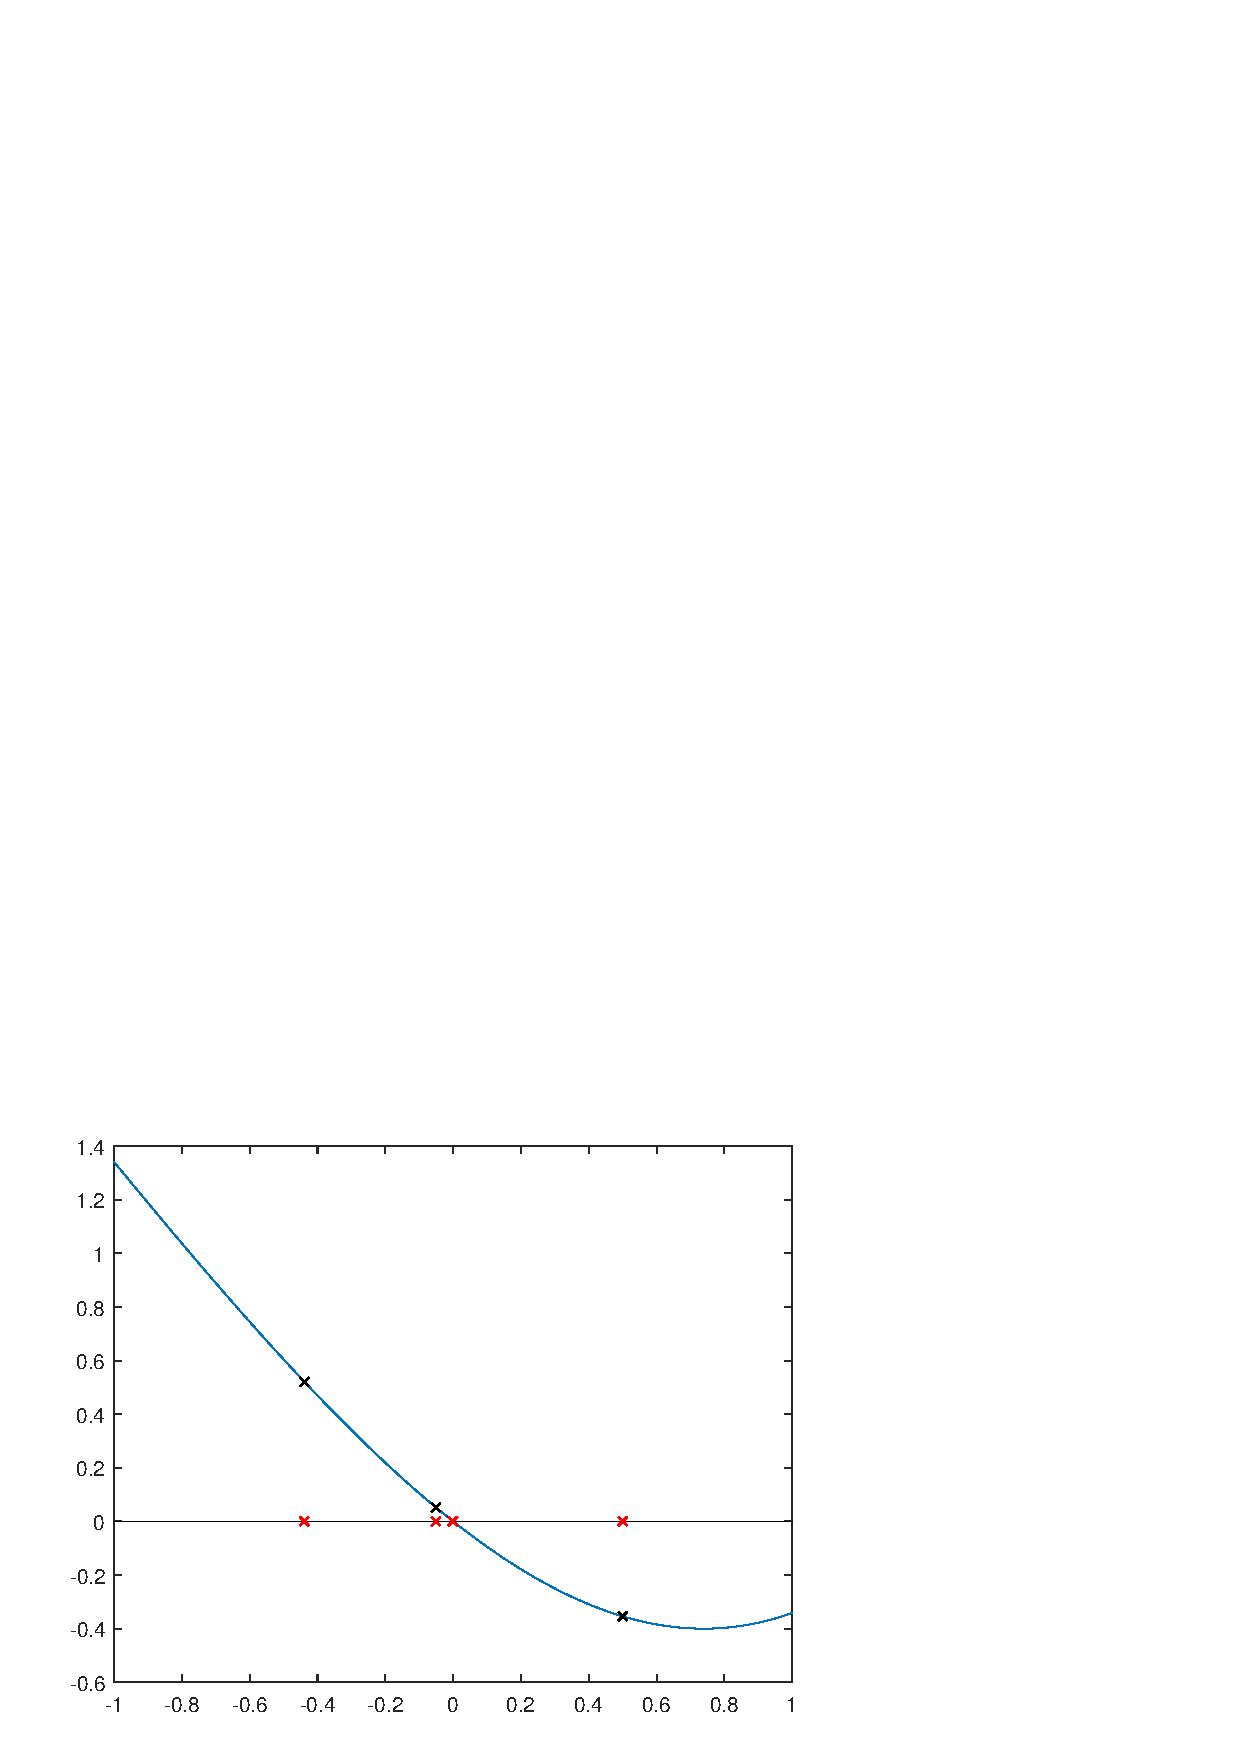
\includegraphics[trim={60 260 50 260},clip, width=.8\linewidth]{./homework3/img/NewtonMethod.pdf}
    \caption{Approximated zeros of a function by the Newton Method. The orange Graph depicts the derivative of the blue function (\ref{eq:fun}).}
    \label{fig:newton}
\end{figure}

\begin{lstlisting}
syms f(x)
f(x) =  ((x.^2)./2) - sin(x);
df = diff(f,x);
ddf = diff(df,x);
x_prev = 0.5;
e = 1;
iterations = 1;
x = -0.5:0.001:1.5;
figure;
plot(x,double(f(x)),'LineWidth',1.2,'DisplayName','f(x)');
hold on
plot(x,double(df(x)),'LineWidth',1.2,'DisplayName','f''(x)');
l = refline([0 0]);
l.Color = [0,0,0];
l.LineStyle = '-';
l.LineWidth = 0.1;
while e >= 1e-5
    x_next = x_prev - (double(df(x_prev))/double(ddf(x_prev)));
    e = abs(x_next - x_prev);  
    plot(x_prev,double(f(x_prev)),'kx');
    plot(x_prev,0,'rx');
    x_prev = x_next;
    iterations = iterations + 1;
end
xlabel('x');
ylabel('y');
print('fig/NewtonMethod.pdf','-dpdf');
\end{lstlisting}